%!TEX root = ../AST208-notes.tex

\section{Electromagnetic radiation is quantized}

Electromagnetic radiation---light---is carried by massless particles known as \emph{photons}. Being massless, they travel at a speed $c$ in all frames.  The energy of a photon depends on its frequency $\nu$: $E_{\nu} = h\nu$. Since $\nu = \lambda/c$, we can also express the energy of a photon as $E_{\lambda} = hc/\lambda$. When matter absorbs or emits radiant energy, it does so by absorbing or emitting photons.

\begin{exercisebox}
On a very dark night, the eye can make out stars down to visual magnitude $V\approx 6$. Given that the sun has $V=-26.71$ and that the flux from the sun in $V$-band is approximately $\val{10^{3}}{\unitstyle{W}/\meter^{2}}$, estimate the radiant flux from this $V=6$ star.  If the $V$ band photons have an average $\lambda = \val{550}{\nano\meter}$, how many photons from this barely visible star enter your pupil and strike your retina each second?
\end{exercisebox}

Suppose we shine a monochromatic (i.e., comprising a single wavelength) beam of light at a tinted piece of glass (sunglasses, for example).  The light that emerges on the other side is the same color---meaning it has the same wavelength---but is dimmer. What are we to make of this? For the exiting light to be dimmer, some of the photons must have been absorbed. But if the photons are indistinguishable, why are only some absorbed? Once we have quantization, we are forced to adopt a probabilistic viewpoint: each photon has a certain probability of being absorbed.

\section{The hydrogen atom}

The electrons bound to an atom or molecule can only occupy states having a discrete set of energies. For example, the electron in a hydrogen atom only has energies
\begin{equation}\label{e.H-levels}
	E_{n} = -\val{13.6}{\eV}\times \frac{1}{n^{2}},
\end{equation}
where $n > 0$ is an integer known as the principal quantum number.  These energies are negative, relative to a free electron.  For example, it takes \val{13.6}{\eV} to remove an electron in its ground state from the atom.

Because the electrons in an atom can only have certain energies, the atom can only absorb or emit light at specific wavelengths, such that the energy of the photon matches the difference in energy between two levels.  For example, a hydrogen atom can absorb a photon of energy
\[
	E_{1\to2} = -\val{13.6}{\eV} \left(\frac{1}{2^{2}} - \frac{1}{1^{2}}\right)
		 = \val{10.2}{\eV}
\]
corresponding to the energy required to move the electron from  $n=1$ to $n=2$.

The wavelengths that can be emitted or absorbed by a hydrogen atom at rest can be found by substituting $E = hc/\lambda$ into equation~(\ref{e.H-levels}):
\begin{equation}
	\lambda_{m\to n} = \lambda_{0}\left(\frac{1}{n^{2}}-\frac{1}{m^{2}}\right)^{-1},
\end{equation}
where $\lambda_{0} = \val{91.2}{\nano\meter}$.
The transitions to the lowest levels are named after their discoverers: Lyman for $m\to1$, Balmer for $m\to2$, Paschen for $m\to3$. A greek letter is used to denote the higher state: for example Lyman $\alpha$ (abbr.\ Ly$\alpha$) means $2\to1$, with $\lambda_{\mathrm{Ly}\alpha} = \val{121.6}{\nano\meter}$.  The first line transition in the Balmer series is $3\to2$, and is designated H$\alpha$: $\lambda_{\mathrm{H}\alpha} = \val{656.3}{\nano\meter}$. The first 50 lines for the Lyman ($m\to1$), Balmer ($m\to2$), and Paschen ($m\to3$) are shown in Fig.~\ref{f.H-spectrum}; note the $4\to3$ transition is outside the plot range.

\begin{figure}[htbp]
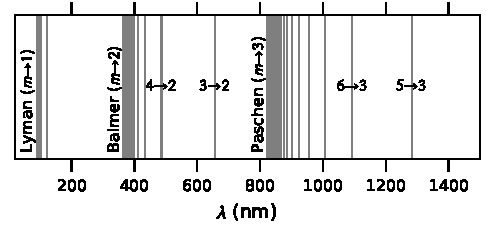
\includegraphics[width=\linewidth]{H-spectrum}
\caption{Spectral lines of neutral hydrogen. 
\label{f.H-spectrum}}
\end{figure}

\section{Diffraction Gratings}

To look at the different wavelengths in the light from a source, we use a diffraction grating, which is a series of fine, closely spaced lines etched on a surface.  When light is projected onto the grating, it is reflected from the lines in all directions.  Along a given direction, the light from two adjacent lines will travel a slightly different distance: if the spacing between lines is $d$, the extra distance traveled from a neighboring line is $d\sin\theta$, where $\theta$ is the angle between the incident and reflected rays. Because of this different path length, a distant detector will in general receive waves of many different phases. When the waves are added together, the peaks and troughs cancel, and the result is that the summed wave is greatly reduced in amplitude.

There are, however, certain directions along which the intensity is maximized. If the extra path length is a multiple of the wavelength then all the waves reach the distant detector so the intensity is bright. That is, at angles satisfying
\begin{equation}
d\sin\theta = m\lambda,
\end{equation}
bright spots are produced.This situation is depicted in Fig.~\ref{f.diffraction-grating} for $m=1$. For each line, the path length differs by one wavelength from its neighbors; as a result, the rays along a direction $\theta$ (at the right of the figure) are in phase.  Since different wavelengths produce their bright spots at different angles, the light is dispersed in wavelength, producing a spectrum.
A good home example of a grating is a compact disk: the tracks on the disk diffract light.

\begin{marginfigure}
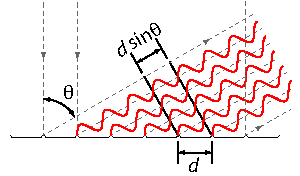
\includegraphics[width=\linewidth]{diffraction-grating}
\caption{A diffraction grating.
\label{f.diffraction-grating}}
\end{marginfigure}

\begin{exercisebox}
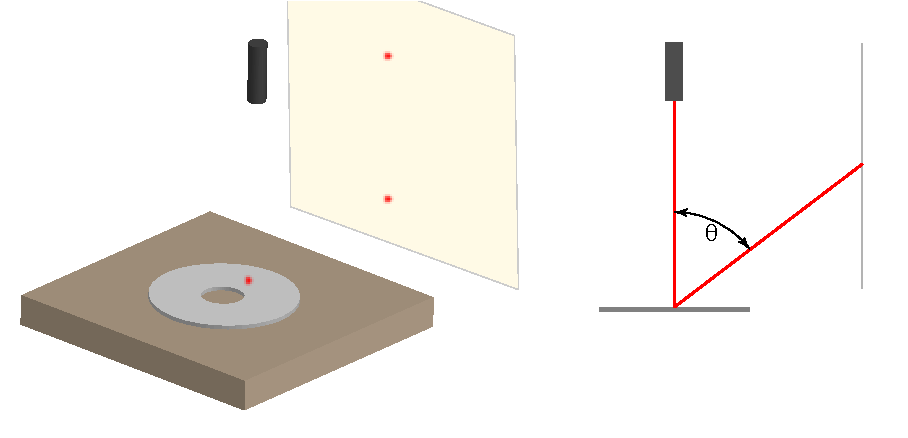
\includegraphics[width=\linewidth]{cd-diffraction-AST208}
You shine a red laser pointer ($\lambda=\val{650}{\nano\meter}$) onto a face-up CD, and observe that two dots appear on a blank screen, as shown above. The laser beam is vertical and the two dots that appear on the screen are at angles $23^{\circ}$ and $52^{\circ}$ from the vertical. There is no other dots appearing. From the information given, calculate the spacing between the tracks on the CD.  Suppose we then shine a green laser pointer ($\lambda=\val{530}{\nano\meter}$) at the disk. At what angles would dots appear?
\end{exercisebox}

For a telescope, there is an additional complication: we don't have a single source, but rather an image of the entire field of view. To restrict our field of view, we overly our grating with a slit, as shown in Figure~\ref{f.slit-and-grating}. The width of the slit is matched to the seeing so that if projects a line of light onto the diffraction grating. The dispersed light thus makes a two dimensional image, with position along the slit along one axis, and wavelength along the other axis.

\begin{figure}[htbp]
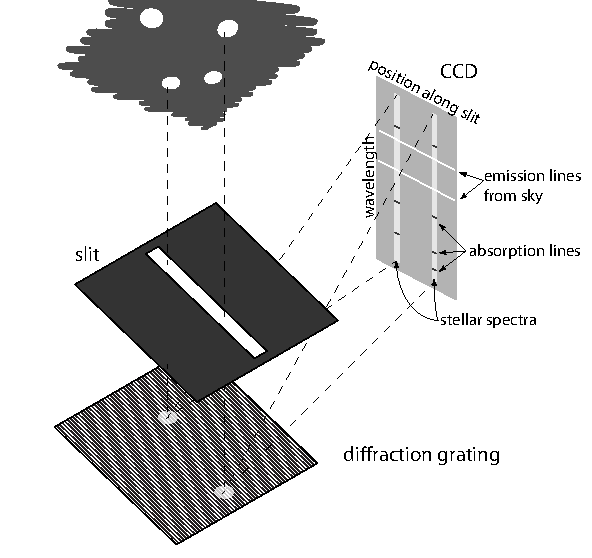
\includegraphics[width=\linewidth]{slit-and-grating}
\caption{Taking a spectrum of an astronomical object.
\label{f.slit-and-grating}}
\end{figure}

\section{Absorption and emission lines}
Now that we are taking spectra, what do we see?  Suppose we look at a tenuous cloud of hot gas, and there is no light source behind this cloud. Because the gas is hot, collisions between atoms will excite electrons into excited states. When these electrons make a transition to the ground state, a photon is emitted. Thus, when we take a spectrum of the light from this cloud, we expect to see a series of discrete, bright lines at those frequencies. This is an \emph{emission line spectrum}. 

Emission lines are also produced in Earth's atmosphere from a variety of sources: for example collisions of molecues with cosmic rays and recombination of ions and electrons that had been photoionized by sunlight.

Conversely, suppose we have gas that is backlit by a strong source of photons---think of the atmosphere of a star. As the photons go through the gas, some are absorbed. Thus, the spectrum is a continuous blend of light, with darker lines corresponding to the absorption in the atmosphere.  This is an \emph{absorption line} spectrum.

When a gas becomes sufficiently dense that it is opaque, meaning that no light gets through it, then the surface emits a broad \emph{continuous spectrum} of light, with the flux peaking at a wavelength that corresponds to the temperature of the gas. The hotter the gas, the shorter the peak wavelength.


\section{The Doppler Shift}\label{s.doppler}

In addition to telling us about the intrinsic properties of the medium producing the spectrum---its temperature, density, and composition---the spectrum can also tell us about its velocity. Because light has wave-like behavior, it has properties in common with other waves you are familiar with, such as sound.  One property that is very useful in astronomy is the \emph{Doppler effect}: the wavelength changes depending on the motion of the source along your line of sight.  To give a concrete example, suppose we have a source that is moving away from us with velocity $v$.  We'll take $v$ positive for motion away from us.\sidenote{The convention here is not universal; in physics texts, $v$ is usually taken as positive if the motion is towards the observer. In that case, replace $v$ with $-v$ in eq.~(\ref{e.doppler0}) below. As always, one must pay attention to the context before using a formula.}

If the source is emitting light with wavelength $\lambda$, then the period (time between successive crests) is $T = \lambda/c$.  In this time $T$, however, the source has moved away from us a distance $vT$. The tail of the wave is therefore not at a distance $\lambda$ from the head, but rather at a distance $\lambda + vT$.  As a result, the wavelength we receive is not $\lambda$, but rather
\begin{equation}\label{e.doppler0}
 \lambda' = \lambda + vT = \lambda + \frac{v}{c}\lambda = \lambda\left(1+\frac{v}{c}\right).
\end{equation}
In deriving this equation, you may have noticed that the speed of the light wave $c$ is unaffected by the motion of the source.  Unlike other waves such as sound, a light wave always moves at a speed $c$ regardless of the motion of either the emitter or the receiver. With light, only the relative speed of the source and observer matters in the expression for the doppler shift.

\begin{figure*}
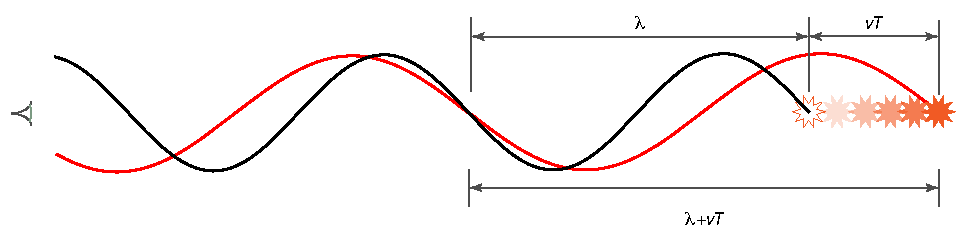
\includegraphics[width=\linewidth]{doppler}
\caption[Schematic of the doppler effect]{Schematic of the doppler effect for a source (red star) moving to the right at speed $v$.}
\label{f.doppler}
\end{figure*}

There is one further modification to equation~(\ref{e.doppler0}).
A consequence of $c$ being a constant is that time passes at different rates for the emitter and receiver.  The period of the wave $T$ is what is measured at the source.  The observer, however, measures that interval of time to be $T/\sqrt{1-v^{2}/c^{2}}$.  Since the wavelength is $\lambda = cT$, this means there is an additional redshift to the wavelength as well.

When these changes are made, the formula for the wavelength observed from a source moving at radial velocity $v$ is
\begin{equation}\label{e.doppler}
\lambda_{\mathrm{obs}} 
 = \lambda_{\mathrm{source}} \left[\frac{1+v/c}{\sqrt{1-v^{2}/c^{2}}}\right].
\end{equation}
In this equation, $v$ is the velocity of the source along the line of sight.
For a source moving towards us, the observed wavelength is shortened; as a result, a line in the middle of the visible spectrum (yellow-green) is shifted toward the blue.  We call this a \emph{blueshift}, irrespective of the actual wavelength of the light.  For a source moving away from us, a line in the yellow-green is shifted toward the red; we term this a \emph{redshift}.

\begin{exercisebox}[Doppler shift of radar beam]
A radar detector used by law enforcement measures speed by emitting a radar beam with frequency \val{22}{\Giga\Hz} and measuring the frequency of the reflected signal.
\begin{enumerate}
\item What is the wavelength $\lambda$ of the radar beam?
\item If a motorist is going \val{40}{\meter/\second} (about 89~miles/hour) away from the officer, what is $\Delta\lambda = \lambda_{\mathrm{motorist}} - \lambda_{\mathrm{officer}}$? What is $\Delta\lambda/\lambda$?
\end{enumerate}
\end{exercisebox}

